% Adapted from the supplied CSIT5760 Final Project Report Template.
% Local tests and Sepolia deployment have separate evidence records.
\documentclass[12pt,a4paper]{report}
\usepackage[a4paper,margin=1in]{geometry}
\usepackage[T1]{fontenc}
\usepackage[utf8]{inputenc}
\usepackage{lmodern,setspace,microtype,xcolor,hyperref,booktabs,array,tabularx,fancyhdr,listings,graphicx,amssymb,amsmath,caption,enumitem,tikz}
\usetikzlibrary{arrows.meta}
\definecolor{linkblue}{RGB}{0,76,153}
\definecolor{codegray}{RGB}{246,247,249}
\definecolor{plotblue}{RGB}{0,78,125}
\definecolor{refundcolor}{RGB}{182,112,35}
\hypersetup{colorlinks=true,linkcolor=linkblue,urlcolor=linkblue,citecolor=linkblue,pdftitle={StreamPay: CSIT5760 Final Project Report},pdfauthor={MA, Yuechen}}
\pagestyle{fancy}\fancyhf{}\lhead{CSIT5760}\rhead{StreamPay Final Project Report}\cfoot{\thepage}\setlength{\headheight}{15pt}
\setstretch{1.12}
\setlength{\parindent}{0pt}\setlength{\parskip}{6pt}
\setlength{\intextsep}{14pt plus 3pt minus 2pt}
\setlength{\textfloatsep}{18pt plus 3pt minus 2pt}
\captionsetup{font=small,skip=6pt}
\captionsetup[table]{position=above,hypcap=false}
\setlist{nosep,leftmargin=*}
\renewcommand{\arraystretch}{1.12}
\newcolumntype{Y}{>{\raggedright\arraybackslash}X}
\newcolumntype{P}[1]{>{\raggedright\arraybackslash}p{#1}}
\newcommand{\file}[1]{\path{#1}}
\setcounter{tocdepth}{0}
\makeatletter
\renewcommand*\l@chapter{\@dottedtocline{0}{0pt}{1.7em}}
\renewcommand\section{\@startsection{section}{1}{\z@}{-2.25ex\@plus-.4ex\@minus-.2ex}{1.1ex\@plus.2ex}{\normalfont\Large\bfseries}}
\renewcommand{\@makechapterhead}[1]{\vspace*{8pt}{\parindent\z@\raggedright\normalfont\LARGE\bfseries\ifnum\c@secnumdepth>\m@ne\@chapapp\space\thechapter\quad\fi #1\par\nobreak\vskip 14pt}}
\renewcommand{\@makeschapterhead}[1]{\vspace*{8pt}{\parindent\z@\raggedright\normalfont\LARGE\bfseries #1\par\nobreak\vskip 14pt}}
\makeatother
\lstdefinelanguage{Solidity}{keywords={pragma,solidity,contract,is,using,for,enum,struct,error,event,address,uint256,bool,bytes,memory,storage,public,private,external,internal,view,pure,immutable,constructor,function,returns,return,if,else,revert,emit,true,false},sensitive=true,comment=[l]{//},morecomment=[s]{/*}{*/},morestring=[b]"}
\lstset{basicstyle=\ttfamily\footnotesize,backgroundcolor=\color{codegray},frame=single,breaklines=true,columns=fullflexible,showstringspaces=false,aboveskip=6pt,belowskip=5pt,captionpos=b}
\renewcommand{\bibname}{References}
\begin{document}
\raggedbottom
\hypersetup{pageanchor=false}
\begin{titlepage}
\centering
\vspace*{1.4cm}
{\LARGE\bfseries CSIT5760\par}
\vspace{0.3cm}
{\Large Blockchain and Smart Contracts\par}
\vspace{1.2cm}
{\Huge\bfseries Final Project Report\par}
\vspace{0.3cm}
{\Large Individual Project\par}
\vfill
\begin{tabularx}{\linewidth}{@{}P{3.4cm}Y@{}}
\toprule
\textbf{Project title} & StreamPay: Prepaid Token Streaming with Cancellation Settlement and Recipient Protection\\
\textbf{Student name} & MA, Yuechen\\
\textbf{Student ID} & 21346213\\
\textbf{Instructor} & Pritom Rajkhowa\\
\textbf{Submission date} & 21 November 2026\\
\textbf{Repository URL} & \url{https://github.com/ycma-nocturne/StreamPay}\\
\textbf{Network} & Ethereum Sepolia\\
\bottomrule
\end{tabularx}
\vfill
{\large Academic Year 2026--2027\par}
\end{titlepage}
\hypersetup{pageanchor=true}
\pagenumbering{roman}

\chapter*{Abstract}
\addcontentsline{toc}{chapter}{Abstract}
StreamPay handles short-term payment agreements with a fixed budget and a time-based schedule. The sender funds an Ethereum escrow at creation. The recipient can withdraw accrued tokens in parts. If the sender cancels, the contract freezes accrual at the cancellation block and reserves the unearned balance for a refund. Each party claims its share separately. The contract uses a fixed demonstration token and tracks the amount owed across streams.

Local validation produced 50 passing tests: 34 contract cases and 16 deployment-tooling cases. Three deterministic campaigns checked 240 actions against an independent integer model. Slither reported five Low timestamp findings and one Informational finding in the assessed scope. Three deployment-tooling fixes passed regression checks. The local demonstration settled a stream at its scheduled end and another after cancellation. The cancellation froze 280,000 raw units for the recipient and reserved 420,000 for the sender. Both accounts collected their shares through separate transactions, reducing the escrow balance and liability to zero.

Both contracts were deployed to Ethereum Sepolia and their source code was verified on Etherscan. The functional tests and settlement demonstration ran on the local Hardhat network.

\tableofcontents

\clearpage
\pagenumbering{arabic}
\chapter{Project Overview}
\section{Project Title}
StreamPay: Prepaid Token Streaming with Cancellation Settlement and Recipient Protection.

\section{Objectives}
The project implements prefunded streams with linear accrual, partial withdrawals and one-time cancellation. The tests check withdrawal limits, cancellation shares and liability backing.

Success means that no recipient can withdraw more than its accrued entitlement, cancellation cannot remove funds already accrued, and either party can collect its cancellation share independently. Tracked unpaid liabilities must remain covered by the escrow's token holdings under the supported token assumptions.

\section{Background and Motivation}
Payment after work leaves a collaborator dependent on a sponsor's willingness and ability to settle. Full advance payment exposes the sponsor if the arrangement ends early. A prepaid stream allocates a fixed budget over time under terms accepted when the stream is created. Sablier provides prior art for streaming and cancellation that preserves vested recipient funds~\cite{sablier,cancelability}. StreamPay uses a fixed test token and separate claims.

A database can calculate accrual. The operator controls the ledger and releases payments. Ethereum escrow publishes the schedule and settlement state, and each party can submit a claim independently.

\section{Scope and Limitations}
The implemented scope includes multiple independent streams, exact prefunding, time-based accrual, recipient withdrawals, sender cancellation, sender refunds, queries, events and command-line interaction. \texttt{MockStreamToken} is a fixed-supply, six-decimal asset with no monetary value. Agreements and account roles in the demonstrations are synthetic.

The scope excludes protocol fees, upgrades, administrator access to funds, other assets, work verification and automatic payouts. Block timestamps determine accrual. Settlement requires transactions and access to the parties' accounts.

\chapter{System Design}
\section{Architecture Overview}
Figure~\ref{fig:architecture} shows how users query contracts and submit transactions through Hardhat scripts. The verification script sends source to Etherscan. Agreement details stay off-chain.

\begin{figure}[htbp]
\centering
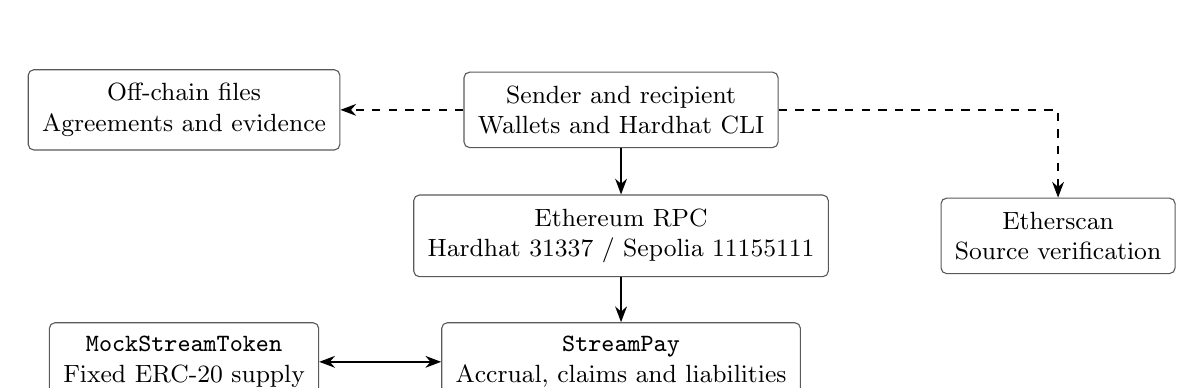
\begin{tikzpicture}[
  box/.style={draw=black!65,rounded corners=2pt,align=center,inner sep=5pt,font=\small},
  link/.style={-{Stealth[length=2mm]},line width=0.6pt}
]
\node[box] (users) at (0,1.6) {Sender and recipient\\Wallets and Hardhat CLI};
\node[box] (network) at (0,0) {Ethereum RPC\\Hardhat 31337 / Sepolia 11155111};
\node[box] (escrow) at (0,-1.6) {\texttt{StreamPay}\\Accrual, claims and liabilities};
\node[box] (token) at (-5.55,-1.6) {\texttt{MockStreamToken}\\Fixed ERC-20 supply};
\node[box] (explorer) at (5.55,0) {Etherscan\\Source verification};
\node[box] (offchain) at (-5.55,1.6) {Off-chain files\\Agreements and evidence};
\draw[link] (users) -- (network);
\draw[link] (network) -- (escrow);
\draw[{Stealth[length=2mm]}-{Stealth[length=2mm]},line width=0.6pt] (escrow) -- (token);
\draw[link,dashed] (users) -- (offchain);
\draw[link,dashed] (users.east) -| (explorer.north);
\end{tikzpicture}
\caption{System architecture.}
\label{fig:architecture}
\end{figure}

\section{User Roles and Access Control}
Roles are assigned by creation: \texttt{msg.sender} becomes the sender and the supplied address becomes the recipient. Neither can be replaced or revoked for an existing stream. There is no contract-owner role.

\begin{tabularx}{\linewidth}{@{}P{2.3cm}Y Y@{}}
\toprule
Role & Permissions & Restriction\\\midrule
Sender & Approve/fund creation; cancel; withdraw refund & Cancellation is once and strictly before the end; refunds require cancellation.\\
Recipient & Withdraw any positive available portion & Always paid to the fixed recipient; cannot redirect or exceed entitlement.\\
Any observer & Read state, availability, status and events & Read access grants no claim authority.\\
\bottomrule
\end{tabularx}

\section{Data and Process Design}
The mapping keys stream IDs to \texttt{Stream} structs. Each struct stores the parties, deposit, times, payments, cancellation flag and frozen accrual. Calls that take an ID reject unallocated IDs. The \texttt{Status} enum represents the derived lifecycle. \texttt{totalLiabilities} tracks the unpaid balance across streams.

\begin{tabularx}{\linewidth}{@{}P{2.2cm}Y@{}}
\toprule
Derived state & Condition and permitted progression\\\midrule
Scheduled & Not cancelled and $t<s$; time leads to Active, or sender cancellation leads to Cancelled.\\
Active & Not cancelled and $s\leq t<e$; time leads to Ended, or sender cancellation leads to Cancelled.\\
Ended & Not cancelled and $t\geq e$; remaining recipient claims stay payable; cancellation is prohibited.\\
Cancelled & Frozen accrual at cancellation; recipient and sender claims remain payable independently.\\
\bottomrule
\end{tabularx}

Figure~\ref{fig:stream-workflow} shows how funding leads to the two settlement paths.

\begingroup
\centering
\captionsetup{hypcap=false}
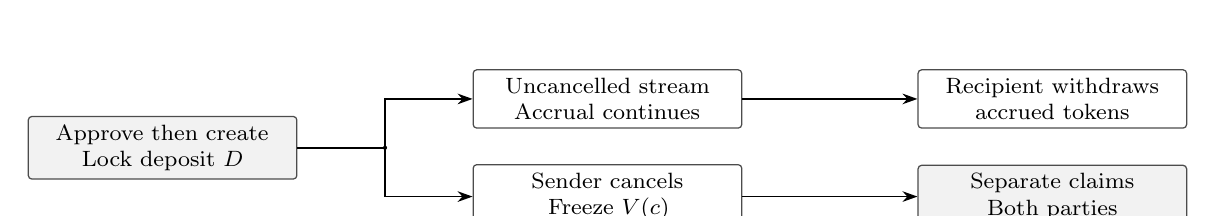
\begin{tikzpicture}[
  workflow node/.style={
    draw=black!70, rounded corners=1.3pt, line width=0.45pt,
    align=center, text width=32mm, inner xsep=3pt, inner ysep=3pt,
    font=\footnotesize
  },
  workflow arrow/.style={-{Stealth[length=1.9mm,width=1.35mm]}, line width=0.6pt}
]
  \node[workflow node, fill=black!5] (fund) at (-5.65,0)
    {Approve then create\\Lock deposit \(D\)};
  \node[workflow node] (accrue) at (0,0.62)
    {Uncancelled stream\\Accrual continues};
  \node[workflow node] (cancel) at (0,-0.62)
    {Sender cancels\\Freeze \(V(c)\)};
  \node[workflow node] (normal) at (5.65,0.62)
    {Recipient withdraws\\accrued tokens};
  \node[workflow node, fill=black!5] (claims) at (5.65,-0.62)
    {Separate claims\\Both parties};

  \coordinate (split) at (-2.825,0);
  \draw[line width=0.6pt] (fund.east) -- (split);
  \fill (split) circle[radius=0.75pt];
  \draw[workflow arrow] (split) |- (accrue.west);
  \draw[workflow arrow] (split) |- (cancel.west);
  \draw[workflow arrow] (accrue.east) -- (normal.west);
  \draw[workflow arrow] (cancel.east) -- (claims.west);
\end{tikzpicture}
\par
\captionof{figure}{Funding and settlement. If the sender cancels at \(c<e\), the recipient can claim \(V(c)-W\) and the sender can claim \(D-V(c)-R\).}
\label{fig:stream-workflow}
\endgroup

\section{Technology Stack}
\begin{tabularx}{\linewidth}{@{}P{4.3cm}Y@{}}
\toprule
Technology / version & Purpose and choice\\\midrule
Solidity / solc-js 0.8.28 & Exact compiler; locally loaded package avoids a separate compiler download.\\
OpenZeppelin Contracts 5.4.0 & Pinned ERC20, SafeERC20, ReentrancyGuard and Math components~\cite{oz}.\\
Hardhat 2.26.3; ethers 6.14.0 & Local execution, scripts and contract interaction.\\
Node.js 24.22.1; pnpm 11.25.0 & Recorded runtime and lockfile-based dependency installation.\\
Hardhat Verify 2.1.3 & Etherscan source verification~\cite{verification}.\\
Slither 0.11.3 & Static analysis~\cite{slither}.\\
\bottomrule
\end{tabularx}

Compilation enables 200 optimizer runs and targets Shanghai. OpenZeppelin's ERC-20 provides the standard balance and allowance logic. \texttt{SafeERC20} handles failed token transfers consistently, \texttt{ReentrancyGuard} blocks nested mutations, and \texttt{Math.mulDiv} calculates elapsed-time accrual at full precision. The escrow still depends on the fixed token's balance and transfer behavior.

\chapter{Smart Contract Details}
\section{Contract Functionality}
\texttt{MockStreamToken} mints $1{,}000{,}000\times10^6$ raw units once to its deployer and exposes six decimals, so 1 SPAY is $10^6$ raw units. It has no public mint function. \texttt{StreamPay} receives the single immutable token address at construction and has no term-editing or rescue interface.

For deposit $D$, start $s$, scheduled end $e$ and block timestamp $t$, cumulative entitlement follows Equation~\eqref{eq:accrual}.
\begin{equation}
V(t)=\begin{cases}
0,&t\leq s,\\
\left\lfloor\dfrac{D(t-s)}{e-s}\right\rfloor,&s<t<e,\\
D,&t\geq e.
\end{cases}
\label{eq:accrual}
\end{equation}
\texttt{Math.mulDiv} computes integer accrual~\cite{oz}. Figure~\ref{fig:accrual-freeze} shows the split at a cancellation block $c$ between $s$ and $e$.

\begin{figure}[!ht]
\centering
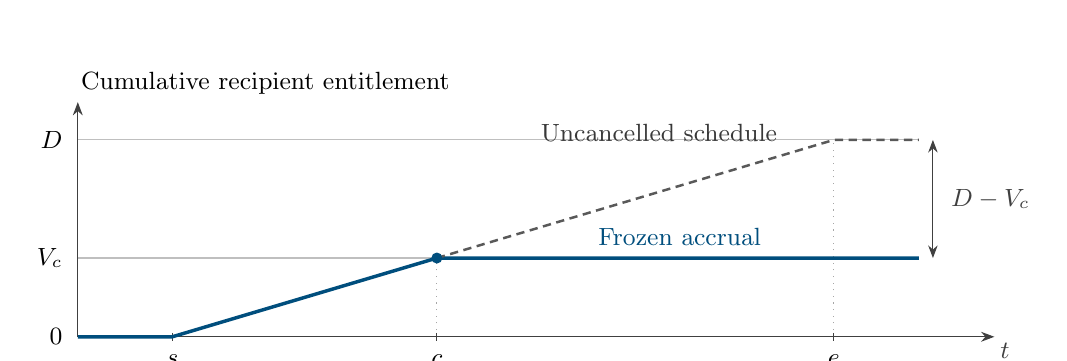
\begin{tikzpicture}[x=1.20cm,y=1.00cm,font=\small,>=Stealth]
  \draw[black!25] (0,2.5) -- (8.9,2.5);
  \draw[black!25] (0,1) -- (3.8,1);
  \draw[black!35,dotted] (3.8,0) -- (3.8,1);
  \draw[black!35,dotted] (8,0) -- (8,2.5);
  \draw[->,black!75] (0,0) -- (9.7,0) node[below right,inner sep=2pt] {$t$};
  \draw[->,black!75] (0,0) -- (0,2.98);
  \node[anchor=south west,inner sep=1pt] at (0,3.04) {Cumulative recipient entitlement};
  \node[left=2pt] at (0,0) {$0$};
  \node[left=2pt] at (0,1) {$V_c$};
  \node[left=2pt] at (0,2.5) {$D$};
  \foreach \position/\symbol in {1/s,3.8/c,8/e}{
    \draw[black!75] (\position,0.05) -- (\position,-0.05);
    \node[below=3pt] at (\position,0) {$\symbol$};
  }
  \draw[plotblue,line width=1.25pt] (0,0) -- (1,0) -- (3.8,1) -- (8.9,1);
  \draw[black!65,densely dashed,line width=0.9pt] (3.8,1) -- (8,2.5) -- (8.9,2.5);
  \fill[plotblue] (3.8,1) circle[radius=2pt];
  \node[plotblue,anchor=south] at (6.37,1.04) {Frozen accrual};
  \node[black!78,anchor=south] at (6.15,2.35) {Uncancelled schedule};
  \draw[black!75,{Stealth[length=1.6mm]}-{Stealth[length=1.6mm]}] (9.05,1) -- (9.05,2.5)
    node[midway,right=3pt] {$D-V_c$};
\end{tikzpicture}
\caption{Schematic of cumulative entitlement. Cancellation freezes $V_c=V(c)$. The bracket marks the sender's total refund allocation.}
\label{fig:accrual-freeze}
\end{figure}

With prior withdrawals $W$ and refunds $R$, the available claims after cancellation are $V_c-W$ for the recipient and $D-V_c-R$ for the sender. Before cancellation, only $V(t)-W$ is available. Each stream maintains $D=W+R+L$, where $L$ is its unpaid liability, and token holdings $H$ cover $\sum L$. Direct donations add surplus without increasing claims.

\clearpage
\section{Interface Description}
Table~\ref{tab:stream-write} lists the write calls. Amounts use raw units and schedules use Unix timestamps. An unknown ID reverts with \texttt{StreamNotFound}. Failed token transfers roll back creation or payout.

\noindent\begin{minipage}{\linewidth}
\small
\captionof{table}{State-changing calls in \texttt{StreamPay}.}
\label{tab:stream-write}
\setlength{\tabcolsep}{5pt}
\begin{tabularx}{\linewidth}{@{}P{4.10cm}P{1.60cm}Y Y@{}}
\toprule
Call & Caller & Result and event & Principal reverts\\\midrule
\texttt{createStream}\newline\texttt{(recipient, amount,}\newline\texttt{start, end)}
  & Any sender
  & Locks the deposit, increases liabilities, returns the new ID and emits \texttt{StreamCreated}.
  & Invalid recipient, zero amount, invalid schedule or failed exact funding.\\
\addlinespace
\texttt{withdraw(id, amount)}
  & Recipient
  & Pays the requested amount, reduces liabilities and emits \texttt{Withdrawn}.
  & Wrong caller, zero amount or amount above the available entitlement.\\
\addlinespace
\texttt{cancel(id)}
  & Sender
  & Freezes accrual, sets the cancellation flag and emits \texttt{Cancelled}.
  & Wrong caller, already cancelled, or block time at or after the end.\\
\addlinespace
\texttt{withdrawRefund(id)}
  & Sender
  & Pays the entire outstanding refund, reduces liabilities and emits \texttt{RefundWithdrawn}.
  & Wrong caller or no refund available.\\
\bottomrule
\end{tabularx}
\end{minipage}

\texttt{createStream} requires $\mathrm{now}\leq s<e$ and a recipient distinct from zero, the sender and the escrow. \texttt{cancel} makes no transfer and leaves total liabilities unchanged.

Anyone can call the views in Table~\ref{tab:stream-read}. The five stream queries take an ID. The last three entries are public getters with no arguments.

\noindent\begin{minipage}{\linewidth}
\small
\captionof{table}{Read-only calls in \texttt{StreamPay}.}
\label{tab:stream-read}
\begin{tabularx}{\linewidth}{@{}P{4.05cm}Y@{}}
\toprule
Call & Return value\\\midrule
\texttt{getStream(id)} & Stored stream record.\\
\texttt{accrued(id)} & Cumulative recipient entitlement.\\
\texttt{withdrawable(id)} & Remaining amount the recipient can claim.\\
\texttt{refundable(id)} & Remaining sender refund. Returns zero before cancellation.\\
\texttt{status(id)} & Derived accrual state. Ended streams may have unpaid claims.\\
\addlinespace
\texttt{token()} & Immutable token address.\\
\texttt{nextStreamId()} & ID for the next stream.\\
\texttt{totalLiabilities()} & Sum of unpaid liabilities across streams.\\
\bottomrule
\end{tabularx}
\end{minipage}

\texttt{MockStreamToken} exposes OpenZeppelin's ERC-20 interface for balances, allowances, approvals and transfers~\cite{oz}.

\clearpage
\section{Important Implementation Decisions}
Pull claims keep the two parties independent: a failed recipient transfer cannot prevent sender cancellation or its refund, and a failed refund cannot prevent the recipient's earned payment. Withdrawal accounting changes before external transfers, and all four mutations use \texttt{nonReentrant}. Exact incoming balance checks reject short or decreasing receipts. The transfer handling follows ERC-20 and Solidity guidance~\cite{erc20,solidity}.

The constructor rejects zero/codeless addresses and failed or malformed \texttt{balanceOf} probes. The escrow uses the fixed demonstration token. Each operation accesses a single stream record.

\section{Representative Code Excerpts}
The following excerpts are exact application source. Complete submitted files remain the source of record; imported OpenZeppelin implementations retain their attribution.

\begin{lstlisting}[language=Solidity,caption={Accrual implementation: contracts/StreamPay.sol, lines 149--154.}]
    function _accrued(Stream storage stream) private view returns (uint256) {
        if (stream.cancelled) return stream.accruedAtCancellation;
        if (block.timestamp <= stream.start) return 0;
        if (block.timestamp >= stream.end) return stream.deposit;
        return Math.mulDiv(stream.deposit, block.timestamp - stream.start, stream.end - stream.start);
    }
\end{lstlisting}

\begin{lstlisting}[language=Solidity,caption={Recipient claim: contracts/StreamPay.sol, lines 79--90.}]
    function withdraw(uint256 id, uint256 amount) external nonReentrant {
        Stream storage stream = _stream(id);
        if (msg.sender != stream.recipient) revert UnauthorizedRecipient(msg.sender);
        if (amount == 0) revert InvalidAmount();
        uint256 available = _accrued(stream) - stream.withdrawn;
        if (amount > available) revert InsufficientWithdrawable(amount, available);

        stream.withdrawn += amount;
        totalLiabilities -= amount;
        token.safeTransfer(stream.recipient, amount);
        emit Withdrawn(id, stream.recipient, amount);
    }
\end{lstlisting}

The first excerpt fixes cancellation entitlement before considering current time. The second binds the caller and destination to the recipient and updates both ledgers before the transfer. Reversion restores those changes when the token transfer fails.

\chapter{Deployment on Testnet}
\section{Deployment Configuration}
Both contracts were deployed to Sepolia on 16 November 2026 UTC. The confirmed receipts and build settings are recorded in \file{deployment/sepolia.json}.

\begingroup\small
\begin{tabularx}{\linewidth}{@{}P{4.1cm}Y@{}}
\toprule
Setting & Recorded configuration / status\\\midrule
Public network & Ethereum Sepolia, chain ID 11155111~\cite{networks}.\\
Local network & Ephemeral Hardhat, chain ID 31337; executed.\\
Compiler / settings & solc-js \path{0.8.28+commit.7893614a.Emscripten.clang}. Optimizer enabled, 200 runs. Shanghai EVM.\\
Libraries / tools & OpenZeppelin 5.4.0; Hardhat 2.26.3; verify plugin 2.1.3.\\
Wallet / signer & Hardhat's local account signer with ethers 6.14.0.\\
Deployer & \path{0x1844c9D82E30a4DE34b4891DbD37Ac51Ba4FF8db}\\
Constructor arguments & \texttt{MockStreamToken} takes none. \texttt{StreamPay} takes the token address shown below.\\
\bottomrule
\end{tabularx}\endgroup

\section{Deployment Information}
\begingroup\small
\begin{tabularx}{\linewidth}{@{}P{3.1cm}Y P{3.35cm}@{}}
\toprule
Contract & Sepolia address & Block and receipt\\\midrule
\texttt{MockStreamToken} & \path{0x61928f9a74879CeE86D2434D65619E18E8c40912} & 12149158, \href{https://sepolia.etherscan.io/tx/0x3f80fea19978d222d5d196fe436abc3c2fd27abddcecdec1caa4a95932c909db}{receipt}\\
\texttt{StreamPay} & \path{0x608E8C677C9Ea162dd776E9a35c4c3eE8323188A} & 12149159, \href{https://sepolia.etherscan.io/tx/0x11b604337b648f9e110a546ad21bcde5dae0b26980d7fbd06c5a3193157d5550}{receipt}\\
\bottomrule
\end{tabularx}\endgroup

The token was deployed at 18:40:36 UTC and the escrow at 18:40:48 UTC on 16 November 2026. Appendix~\ref{app:sepolia-evidence} gives the full transaction hashes.

\section{Etherscan Verification}
\label{sec:etherscan-verification}
\texttt{pnpm verify:sepolia} checked the build settings, source hashes, deployed bytecode and escrow token address. Hardhat Verify submitted the standard JSON input, compiler identifier \path{v0.8.28+commit.7893614a} and encoded constructor arguments~\cite{verification}. The contracts use no externally linked libraries.

Verification was recorded on 16 November 2026 at 18:46:32 UTC for \href{https://sepolia.etherscan.io/address/0x61928f9a74879CeE86D2434D65619E18E8c40912#code}{\texttt{MockStreamToken}} and 18:49:22 UTC for \href{https://sepolia.etherscan.io/address/0x608E8C677C9Ea162dd776E9a35c4c3eE8323188A#code}{\texttt{StreamPay}}. Receipt, bytecode and compiler input checks are in \file{deployment/sepolia-evidence.json}.

\chapter{Test Cases and Validation}
\label{ch:local-tests}
\section{Testing Environment}
Tests used Hardhat 2.26.3 on local chain 31337 with Mocha 10.8.2 and Chai 4.5.0. The fixtures use separate accounts, controlled timestamps, raw token units and a BigInt reference model. All 50 tests passed: 6 creation, 12 settlement, 16 adversarial and accounting, and 16 tooling cases.

Run \texttt{pnpm compile}, \texttt{pnpm test:record}, \texttt{pnpm matrix} and \texttt{pnpm demo}. The matrix in \file{docs/test-matrix.md} records expected and observed outcomes. The raw results retain source and test hashes~\cite{guideline}.

\section{Test-Case Summary}
Table~\ref{tab:validation-cases} summarizes representative cases. All listed cases passed.

\noindent\begin{minipage}{\linewidth}
\small
\captionof{table}{Representative validation cases.}
\label{tab:validation-cases}
\begin{tabularx}{\linewidth}{@{}P{2.05cm}P{4.55cm}Y@{}}
\toprule
Case & Preconditions and input & Expected and observed outcome\\\midrule
T-C03 & Deposit 100 over 10 s. Query $s-1,s,s+1,e-1,e$. & Accrual $0,0,10,90,100$. States progress from Scheduled to Active to Ended.\\
T-S03 & Deposit 100 over 100 s. Claim zero, then 22 at offset 21. & Zero and excessive claims revert. Withdrawals stay at 0 and liability stays at 100.\\
T-S10/11 & Deposit 100, pay 10, cancel at offset 40. Try both claim orders. & Both orders yield 40 total to the recipient, 60 refund, zero liability and Cancelled status.\\
T-S12 & Deposit 7 over 5 s. Query at $0,1,2,4,5$ and claim. & Accrual $0,1,2,5,7$. All seven units are paid.\\
T-A04/05 & Cancel 100 at offset 40. Fail one party's transfer. & The failed transaction rolls back. The other party receives the 60 refund or 40 earned share.\\
T-A08--12 & Attempt nested mutations with token callbacks. Propagate one failure. & The guard reverts with \texttt{0x3ee5aeb5}. Propagating the failure restores both streams and balances.\\
T-A13 & Four deposits total 117. Donate 31 and interleave claims and cancellation. & Recipient 57, refund 60, liability 0, surplus 31.\\
\bottomrule
\end{tabularx}
\end{minipage}

Other cases cover invalid inputs, failed funding, cancellation boundaries, repeat actions, rollback and a one-unit payout. T-A07 checks accrual on a deposit of $2^{255}+7$.

\clearpage
\section{Test Evidence}
The deterministic campaigns compare expected errors, balances, storage and invariants after every action. Each seed ran 80 actions across four streams. Table~\ref{tab:campaigns} shows the final balances.

\noindent\begin{minipage}{\linewidth}
\small
\captionof{table}{Final balances for the three deterministic campaigns.}
\label{tab:campaigns}
\begin{tabularx}{\linewidth}{@{}P{2.5cm}r r r Y@{}}
\toprule
Seed & Actions & Liability & Holdings & Observed surplus\\\midrule
17 & 80 & 2 & 51 & 49\\
5760 & 80 & 1004 & 1166 & 162\\
21346213 & 80 & 77 & 196 & 119\\
\bottomrule
\end{tabularx}
\end{minipage}

Stream 1 accrued 200,000 raw units before any transfer, then paid 400,000 and 600,000. Figure~\ref{fig:cancelled-settlement} follows stream 2. The final recipient balance was 1,280,000, and escrow balance and liabilities were zero.

\noindent\begin{minipage}{\linewidth}
\centering
\captionsetup{hypcap=false}
% Heights are in 10^3 raw units. Allocations are derived from the local demo events.
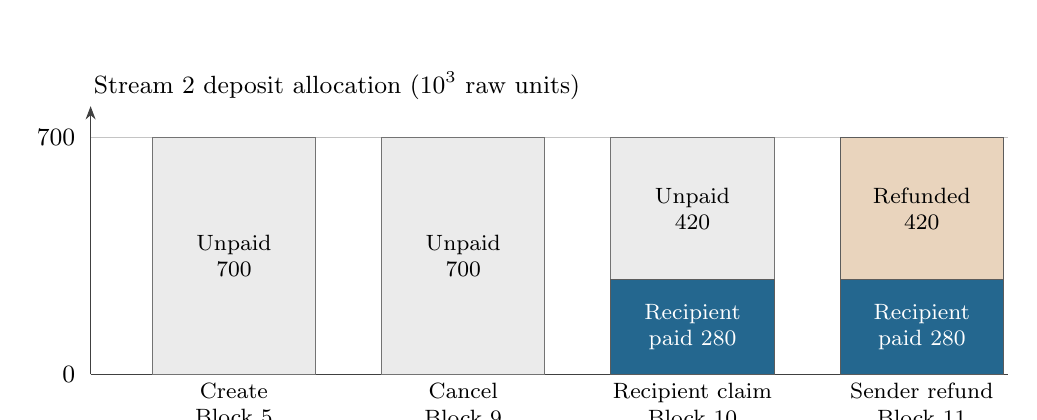
\begin{tikzpicture}[x=1.82cm,y=0.0043cm,font=\small,>=Stealth]
  \draw[black!23] (0,700) -- (6.4,700);
  \draw[->,black!75] (0,0) -- (0,792);
  \draw[black!75] (0,0) -- (6.4,0);
  \node[anchor=south west,inner sep=1pt] at (0,802) {Stream 2 deposit allocation ($10^3$ raw units)};
  \node[left=2pt] at (0,0) {0};
  \node[left=2pt] at (0,700) {700};
  \foreach \xcoord/\paid/\refund/\unpaid/\block/\tx in {
      1/0/0/700/5/{Create},
      2.6/0/0/700/9/{Cancel},
      4.2/280/0/420/10/{Recipient claim},
      5.8/280/420/0/11/{Sender refund}} {
    \pgfmathsetmacro{\leftedge}{\xcoord - 0.57}
    \pgfmathsetmacro{\rightedge}{\xcoord + 0.57}
    \pgfmathsetmacro{\refundtop}{\paid + \refund}
    \ifdim\unpaid pt>0pt
      \draw[fill=black!8,draw=black!55] (\leftedge,\refundtop) rectangle (\rightedge,700);
      \pgfmathsetmacro{\labely}{\refundtop + \unpaid/2}
      \node[align=center,font=\footnotesize] at (\xcoord,\labely)
        {Unpaid\\\unpaid};
    \fi
    \ifdim\paid pt>0pt
      \draw[fill=plotblue!86,draw=black!64] (\leftedge,0) rectangle (\rightedge,\paid);
      \pgfmathsetmacro{\labely}{\paid/2}
      \node[align=center,text=white,font=\footnotesize] at (\xcoord,\labely)
        {Recipient\\paid \paid};
    \fi
    \ifdim\refund pt>0pt
      \draw[fill=refundcolor!30,draw=black!64] (\leftedge,\paid) rectangle (\rightedge,\refundtop);
      \pgfmathsetmacro{\labely}{\paid + \refund/2}
      \node[align=center,font=\footnotesize] at (\xcoord,\labely)
        {Refunded\\\refund};
    \fi
    \node[align=center,anchor=north,font=\footnotesize,inner sep=3pt] at (\xcoord,0)
      {\tx\\Block \block};
  }
\end{tikzpicture}
\captionof{figure}{Stream 2 accounting on local Hardhat chain 31337. Cancellation at 40\% fixes the two claims. The unpaid amount falls as each party collects its share. The allocations use events in \texttt{evidence/local-demo.json}.}
\label{fig:cancelled-settlement}
\end{minipage}

\noindent\begin{minipage}{\linewidth}
\small
\captionof{table}{Gas used by the local demonstration.}
\label{tab:local-gas}
\begin{tabularx}{\linewidth}{@{}Y r Y r@{}}
\toprule
Local operation & Gas used & Local operation & Gas used\\\midrule
Token deployment & 549706 & Escrow deployment & 972003\\
Approve two streams & 46330 & Create first stream & 215554\\
Create second stream & 176554 & Partial withdrawal & 100315\\
Final withdrawal & 65394 & Cancellation & 80385\\
Cancelled recipient claim & 78238 & Sender refund & 68524\\
\bottomrule
\end{tabularx}
\end{minipage}

\chapter{Smart Contract Security Audit}
\section{Audit Scope and Methodology}
The review covered \texttt{StreamPay.sol}, \texttt{MockStreamToken.sol}, and the deployment and verification scripts. It combined Slither 0.11.3, source inspection and local tests.

Slither analyzed 17 compiled contracts with 100 detectors. After filtering dependencies and test fixtures, it reported five Low findings and one Informational finding. The analysis command and the interpretation are in \file{audit/security-review.md}.

\section{Findings Summary}
\begingroup\small
\begin{tabularx}{\linewidth}{@{}P{1.8cm}Y Y@{}}
\toprule
ID / severity & Finding and impact & Response and evidence\\\midrule
S01--S05 / Low & Timestamp dependence in creation, withdrawal, cancellation, status and accrual. Transaction time affects entitlement and boundary behavior. & Retained as intended semantics. Exact-boundary, cancellation and rounding tests passed; coarse-clock and ordering limitations remain.\\
S06 / Informational & Constructor low-level \texttt{staticcall} probes token \texttt{balanceOf}. A well-formed response cannot establish trustworthy token behavior. & Call success and exact 32-byte response are checked. Failed/malformed probes reject in T-C02; fixed-token scope remains.\\
\bottomrule
\end{tabularx}\endgroup

The deployment tooling review identified three findings rated Important.

\begingroup\small
\begin{tabularx}{\linewidth}{@{}P{1.2cm}Y Y@{}}
\toprule
ID & Finding / impact / affected area & Remediation / retest / status\\\midrule
R1 & Runtime provenance checks could accept unrelated bytecode with a matching manifest hash. & Compare build inputs, reconstruct every immutable occurrence and query \texttt{token()}. T-D11/T-D16 passed. Closed.\\
R2 & A metadata RPC failure could discard a confirmed deployment receipt. & Save address, hash and block before fetching metadata. Mark failed metadata reads incomplete. T-D12/T-D14 passed. Closed.\\
R3 & Retrying a public deployment could overwrite an earlier receipt. & Refuse overwrites before broadcasting, with an exception for the empty deferred marker. T-D13/T-D15 passed. Closed.\\
\bottomrule
\end{tabularx}\endgroup

The executed matrix records the outcomes of regression cases T-D11 through T-D16.

\clearpage
\section{Manual Security Review}
Authorization checks bind every claim and cancellation to the fixed party. Positive and bounded claims, cumulative ledgers and one-time cancellation reject repeated collection. Cancelled accrual is frozen before later claims. The supported token balance delta is checked before allocating IDs; liabilities change only with successful funding or payout. The independent model and four-stream cases check conservation and donation surplus.

All four mutations use \texttt{nonReentrant}. Withdrawals and refunds update accounting before transferring tokens. Creation validates the actual balance increase before it records the liability. The callback tests distinguish role checks from reentrancy protection. Failed transfers roll back accounting, and separate claims limit cross-party blocking. The escrow has no payable interface or NFT handling. Per-stream operations avoid loops over all streams, though token or network failure can still block a transfer.

Block time and transaction ordering affect the cancellation split. Parties must verify the address and schedule before funding. Lost keys and direct donations have no recovery path. The public chain exposes transaction addresses, amounts and times. Agreement text stays off-chain.

\chapter{Conclusion and Future Work}
\section{Conclusion}
StreamPay implements prepaid token streaming and cancellation settlement. Both Sepolia deployments passed Etherscan source verification. The recipient's accrued share is preserved at cancellation, sender refunds are separate, and stream liabilities remain inspectable. The retained runs show 50 passing tests and 240 reference-model actions. The local demonstration records complete settlement and measured transaction gas.

The security work interprets six Slither findings and documents three corrected tooling issues. The RPC failure in R2 showed why the script saves each confirmed receipt before requesting extra metadata. Cancellation shares depend on the block timestamp at confirmation, and the escrow supports one fixed test token.

\section{Future Work}
A signing screen could use a wallet connection and the existing read functions over RPC to show the fixed terms and estimate both cancellation shares before signing. The estimate would reflect the latest block timestamp.

\begin{thebibliography}{99}
\raggedright
\addcontentsline{toc}{chapter}{References}
\bibitem{guideline} CSIT5760. \textit{Individual Project Guidelines, Academic Year 2026--2027} and supplied \textit{Final Project Report Template}. Course-provided documents, November 2026.
\bibitem{sablier} Sablier. \textit{Lockup Overview}. \url{https://docs.sablier.com/concepts/lockup/overview}. Accessed 7 November 2026.
\bibitem{cancelability} Sablier. \textit{Cancelability}. \url{https://docs.sablier.com/concepts/cancelability}. Accessed 7 November 2026.
\bibitem{erc20} Ethereum Improvement Proposals. \textit{ERC-20: Token Standard}, EIP-20. \url{https://eips.ethereum.org/EIPS/eip-20}. Accessed 7 November 2026.
\bibitem{oz} OpenZeppelin. \textit{Contracts v5.4.0}: ERC20, SafeERC20, ReentrancyGuard and Math. \url{https://github.com/OpenZeppelin/openzeppelin-contracts/tree/v5.4.0/contracts}. Accessed 7 November 2026.
\bibitem{solidity} Solidity. \textit{Security Considerations}, v0.8.28. \url{https://github.com/ethereum/solidity/blob/v0.8.28/docs/security-considerations.rst}. Accessed 7 November 2026.
\bibitem{slither} Trail of Bits. \textit{Slither}, v0.11.3. \url{https://github.com/crytic/slither/tree/0.11.3}. Accessed 7 November 2026.
\bibitem{networks} Ethereum.org. \textit{Networks: Sepolia}. \url{https://ethereum.org/developers/docs/networks/}. Accessed 7 November 2026.
\bibitem{verification} Nomic Foundation. \textit{Hardhat 2: hardhat-verify}. \url{https://v2.hardhat.org/hardhat-runner/plugins/nomicfoundation-hardhat-verify}. Accessed 7 November 2026.
\end{thebibliography}

\clearpage
\appendix
% Keep the template's five appendix chapters together without forced blank space.
\begingroup
\let\clearpage\relax
\makeatletter
\renewcommand{\@makechapterhead}[1]{{\parindent\z@\raggedright\normalfont\normalsize\bfseries\@chapapp\space\thechapter\quad #1\par\nobreak\vskip 5pt}}
\renewcommand{\@makeschapterhead}[1]{{\parindent\z@\raggedright\normalfont\normalsize\bfseries #1\par\nobreak\vskip 5pt}}
\makeatother
\chapter{Complete Solidity Source Code}
See \file{contracts/MockStreamToken.sol} and \file{contracts/StreamPay.sol} for the complete source and license notices. Section~\ref{sec:etherscan-verification} links to both verified sources. Source hashes accompany the tests, local demonstration and Sepolia deployment records.

\chapter{Deployment Scripts and Configuration}
\begingroup\raggedright
The build is pinned in \file{hardhat.config.cjs}, \file{package.json} and \file{pnpm-lock.yaml}. The operational scripts are \file{scripts/deploy.cjs}, \file{scripts/verify.cjs}, \file{scripts/interact.cjs} and \file{scripts/lib/deployment.cjs}. The README gives build, test and interaction commands. Scripts read credentials from the local environment.\par
\endgroup

\chapter{Test Code and Selected Outputs}
\begingroup\raggedright
The files \file{creation.test.cjs}, \file{settlement.test.cjs}, \file{adversarial.test.cjs} and \file{accounting.test.cjs} under \file{tests/} contain the 34 contract cases. \file{tests/tooling.test.cjs} supplies 16 tooling cases. \file{tests/support/reference.cjs} implements the independent integer model. Expected/actual case records are in \file{docs/test-matrix.md}; raw results, logs and all campaign steps are in \file{evidence/test-results.json}, \file{evidence/tests.txt} and \file{evidence/random-traces.json}.\par\endgroup

\chapter{Security-Analysis Output}
\file{audit/slither.json} contains the analyzer output. \file{audit/security-review.md} records the command, findings and fixes. Cases T-D11 through T-D16 in \file{docs/test-matrix.md} record the tooling retests.

\newpage
\chapter{Etherscan and Transaction Evidence}
\label{app:sepolia-evidence}
\file{deployment/sepolia.json} records the deployment receipts, runtime code hashes, verification responses and verified-source URLs. \file{deployment/sepolia-evidence.json} records the independent receipt, bytecode and source checks. The hashes below link to the Sepolia transactions on Etherscan.

\begingroup\footnotesize
\begin{tabularx}{\linewidth}{@{}P{2.9cm}Y@{}}
\toprule
Contract & Sepolia address and deployment transaction hash\\\midrule
\texttt{MockStreamToken} & \path{0x61928f9a74879CeE86D2434D65619E18E8c40912}\newline\href{https://sepolia.etherscan.io/tx/0x3f80fea19978d222d5d196fe436abc3c2fd27abddcecdec1caa4a95932c909db}{\nolinkurl{0x3f80fea19978d222d5d196fe436abc3c2fd27abddcecdec1caa4a95932c909db}}\\
\texttt{StreamPay} & \path{0x608E8C677C9Ea162dd776E9a35c4c3eE8323188A}\newline\href{https://sepolia.etherscan.io/tx/0x11b604337b648f9e110a546ad21bcde5dae0b26980d7fbd06c5a3193157d5550}{\nolinkurl{0x11b604337b648f9e110a546ad21bcde5dae0b26980d7fbd06c5a3193157d5550}}\\
\bottomrule
\end{tabularx}\endgroup

\file{evidence/local-demo.json} contains the separate Hardhat chain 31337 receipts, events and balances for the local functional demonstration.

\chapter*{Final Submission Checklist}
\addcontentsline{toc}{chapter}{Final Submission Checklist}
\begin{itemize}
\item Contents and cross-references checked.
\item Source and runtime bytecode matched for both verified Sepolia contracts.
\item Compiler, optimizer and EVM settings recorded.
\item Expected and actual test results recorded.
\item Audit findings interpreted and applicable fixes retested.
\item README covers installation, build, test, deployment and interaction.
\item Sepolia addresses, transaction hashes and verified-source links recorded.
\item Credentials and dependency directories excluded from the archive.
\end{itemize}
\endgroup
\end{document}
